\chapter{Parameter Inference with Bifurcation Diagrams}
\label{chapter:inference}
\begin{music}
    \parindent10mm \instrumentnumber{1} \setstaffs1{1} 
    \generalmeter{\meterfrac44} \generalsignature{2}
    \startextract
            \notes \ql j \ql i \Qqbl ieji \en
        \bar \zw{m*} \bar 
            \notes \ql i \qu h \Qqbu hdih \en
        \bar \zw{l*} 
    \zendextract
\end{music}
\epigraph{\textit{the melody that will draw you into the infinite darkness}}{Nocturne of Shadow --- Ocarina of Time}

\section{Preface}
The novel inference method presented in this chapter addresses the specific limitations encountered during the interdisciplinary collaboration in synthetic developmental biology presented in Chapter \ref{chapter:double-exclusive} and lays the foundations for machine learning methods that leverage bifurcation theory. These methods would be relevant in fields where modelling and designing qualitative changes in behaviour is important, observations are scarce and have experiments with highly variable outcomes.

In Chapter \ref{chapter:double-exclusive} the genetic engineers wanted to design synthetic \textit{E. Coli} with a bistable cusp bifurcation with respect to two input signals as shown in Figure \ref{figure:double-exclusive:bistability}. The qualitative design goal was bistability in a region where both signals are present beyond some threshold concentration and monostable otherwise. The next step would have been to engineer an oscillatory region in the input signals --- a Hopf bifurcation. Combining these two designs could have lead to a candidate genetic circuit for forming self-organised patterns across the bacterial colony.

The hierarchical monte-carlo approach --- details of which can be found in Appendix \ref{appendix:double-exclusive:inference} --- enabled the incorporation of knowledge from subsystems and variants of the synthetic \textit{E. Coli} under one model, in an effort to guide genetic engineers through a high dimensional design space towards their design goals. Model parameters were estimated using time-course fluorescence microplate measurements that included information about dynamical transients and colony growth in liquid culture as shown in Figure \ref{fig:microplate-data}. The biological design goals, however, were in state-space rather than the time-domain and are observed in flow cytometry measurements of colonies in exponential phase as shown in Supplementary Figure \ref{figure:double-exclusive:flow-hysteresis}. The disconnect between the domain that the data lives in and the domain of the design goals poses the risk of over-fitting the model on undesired information that exists in the data domain.

In this early days of this thesis, we investigated whether it was possible to transform the time-domain data into the same domain that the design goals lived in: the state-space. This approach, and related works, are discussed in Section \ref{section:field-inference} and can in principle be used with the microfluidic fluorescence microscopy data shown in Figure \ref{figure:double-exclusive:bistability}c for parameter inference. However, the accuracy of the cell trajectories was limited by cell segmentation and tracking algorithms. Initial investigations into this approach also suggested that trajectories need to be of sufficient temporal resolution and sampled from a wide variety of initial conditions. Such data is not widely available and ultimately we decided to focus on a method that could be used with a well-known workhorse in biomedical research: flow cytometry.

Section \ref{section:flow-calculations} describes an experimental design for flow cytometry for the purposes of extracting bifurcation information from cells. The experiments were designed and performed by \textbf{Paul Grant} and \textbf{Valerie Coppard}. Circling back to the original design goals, Section \ref{section:hopf-inference} illustrates how the \textit{bifurcation measure}, introduced in the incorporated publication in Sections \ref{inference:abstract} --- \ref{inference:acknowledgements}, can be extended for Hof bifurcations. \textbf{Grisha Szep} prepared the manuscript, designed the cost function, derived mathematical results, wrote and released the Julia package under the supervision of \textbf{Neil Dalchau} and \textbf{Attila Czicasz-Nagy}.

\subsection{State Field Geometry in Trajectory Data}
\label{section:field-inference}

Consider we are given $K$ cell trajectories $\mathcal{D}_1$, $\mathcal{D}_2$ ... $\mathcal{D}_K$, each containing $N$ noisy observations of the state of the cell. Let the cell state be represented by state vector $u(t)\in\Reals^N$ which is hypothesized to obey a set of ordinary differential equations of the form \eqref{eq:odes}. Instead of integrating the equations \eqref{eq:odes} we would find an estimate for the derivative of the trajectories $\hat{f}$.

This is known as the \textit{smoothing} step \cite{Gugushvili2012Smoothing} should be done using unsupervised methods, for example with Gaussian Process Regressors \cite{Seeger2004GaussianLearning.} as shown in in Figure \ref{fig:inferred-cycles}. This requires the inversion of an $K'\times K'$ data matrix where $K':=\sum_k |\mathcal{D}_k|$ is the total number of trajectory data points. This has a computational complexity $K'^3$ which is only tractable with sparse datasets.

Let the region $\partial\mathcal{D}$ be a boundary defined by the Delaunay tessellation of the input data. Let us define the estimate $\hat f$ only within the region $\partial\mathcal{D}$ so that there are no extrapolation artefacts. For the Gaussian Process approach the estimate would be
\begin{equation}
    \hat{f}(u)\sim
        \mathcal{N}(\,\mu(u) ,\Matrix{\Sigma}(u)\,)
    \quad\mathrm{for}\quad u\in\partial\mathcal{D}
\end{equation}
\noindent where at any given state $u$ the field estimate $\hat{f}$ is generated by Gaussian distributions of mean vector $\mu$ and covariance matrix $\Matrix{\Sigma}$.Solving for these requires a choice of matrix-valued kernel function $\Matrix{K}(u,v)$ which encodes our knowledge about the local structure of the field. Sophisticated kernels for learning vector fields exist \cite{Fuselier2017ADecompositions} for decomposing fields in conservative and solenoidal components, which aid in localising fixed points and cycles.

\begin{Figure}
    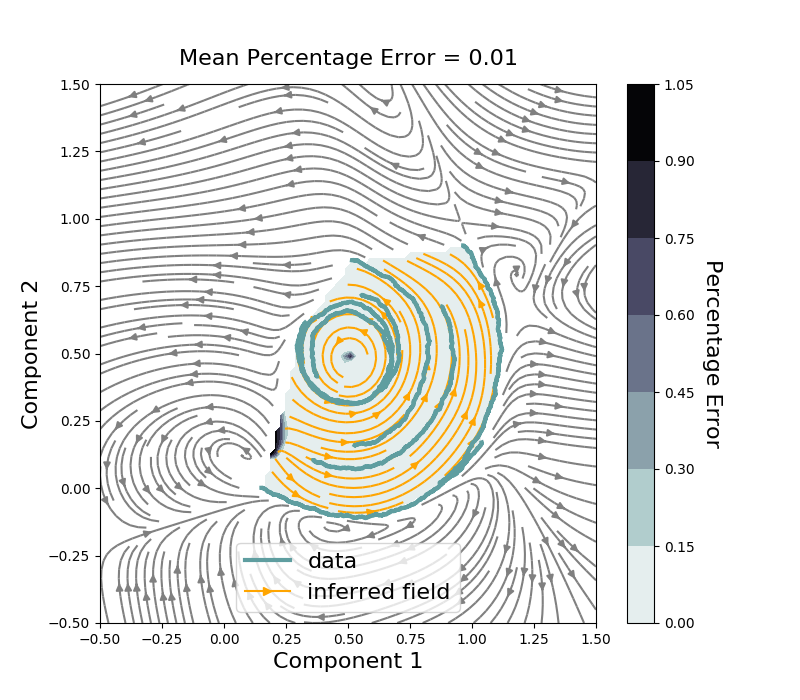
\includegraphics[width=125mm]{figures/cycle-2.png}
    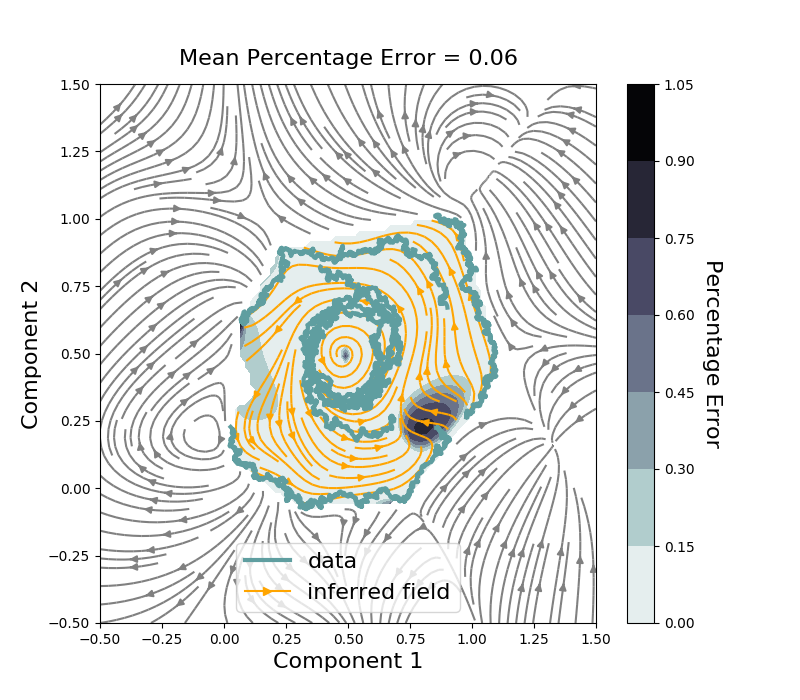
\includegraphics[width=125mm]{figures/cycle-1.png}
    \caption{Gaussian process regressors estimating derivative of the trajectories $\hat{f}$ from example trajectory datasets $\mathcal{D}_1$ ... $\mathcal{D}_K$ with varying signal to noise ratios. Interpolation error $E$ is shown as a heatmap; extrapolation fails}
    \label{fig:inferred-cycles}
\end{Figure}

The simplest choice of kernel assumes the components are independent and have a finite correlation length $\gamma$, such as Gaussian radial basis functions. Here $\Matrix{I}$ is the identity matrix and the hyperparameter $\gamma$ has to be optimised.
\begin{equation}
    \Matrix{K}(\Vector{u},\Vector{v}) = \Matrix{I}\,\mathbb{e}^{-\gamma|\Vector{u}-\Vector{v}|^2}
\end{equation}

The second step is called \textit{matching} where the estimated field $\hat{f}$ is used as an optimisation target against some parametrised function $\rates$ with unknown parameters $\theta$.

In our setting we would like to match the geometry of the field but not its magnitude; in this sense we are focusing on the qualitative aspects of the dynamics of a set of differential equations, rather than the quantitative dynamics or kinetics. This could be achieved with the following objective function
\begin{equation}
    \mathcal{L}(\theta|\mathcal{D}) := e^{-\frac{\hat{f}\cdot\rates}
    {|\hat{f}||\rates|}}
\end{equation}
where the cost is minimal when the data derivative $\hat{f}$ and the parametrised model $\rates$ point in the same direction and maximal when they point in opposing directions.

Although we are getting close to focusing on qualitative features of a model, this objective function is still sensitive to the locations and shapes of fixed point and limit cycles. What if we cared about even higher-level features such as the number of fixed points? Or perhaps whether a system oscillates or not? This is where the language of bifurcation theory described in Chapter \ref{chapter:background} is optimally suited for this task, but fist we need to discuss how to set up experiments to detect bifurcations from flow cytometry data.

\subsection{Bifurcations in Flow Cytometry Data}
\label{section:flow-calculations}



\subsection{Extending the Bifurcation Measure for Limit Cycles}
\label{section:hopf-inference}

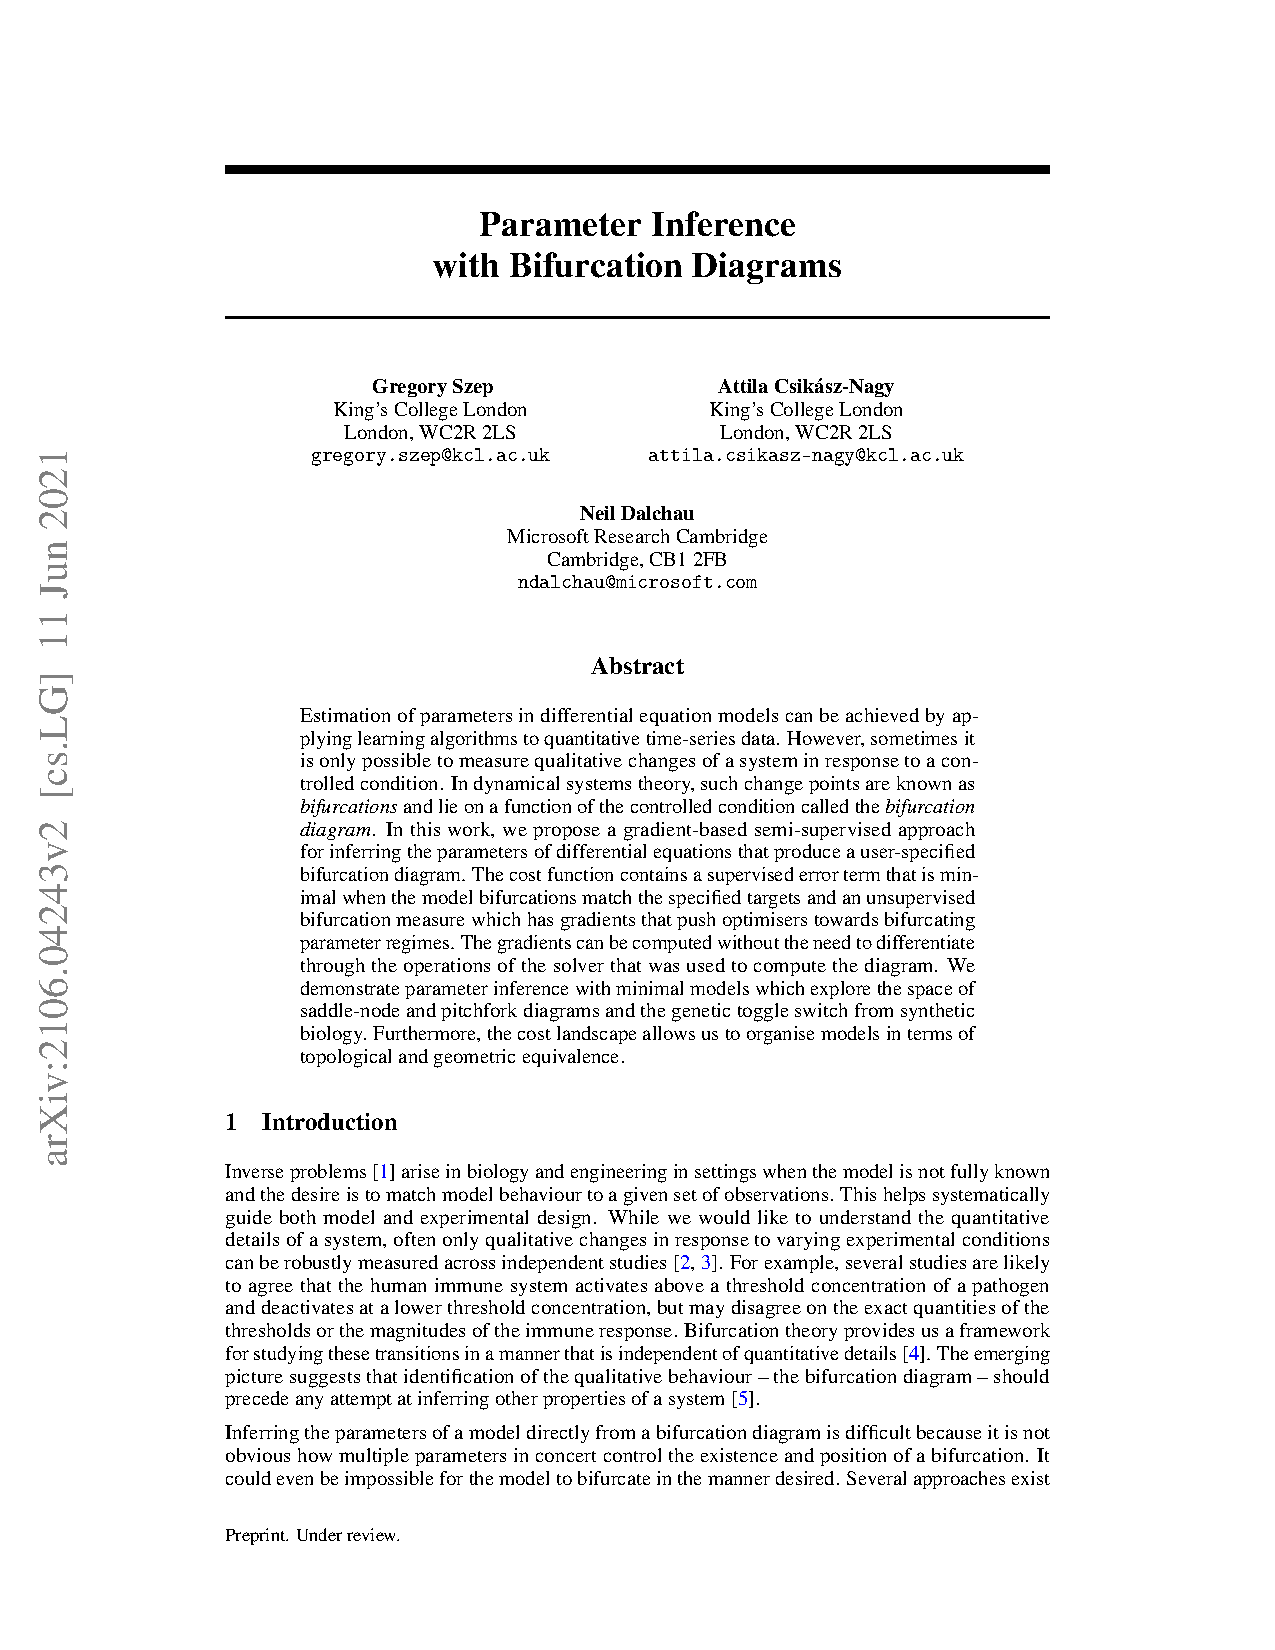
\includepdf[pages=1-11, offset=75 -95, scale=0.85, frame,
        clip,trim=31mm 21mm 31mm 21mm,
        pagecommand={}, addtotoc={
        1,section,1,Abstract,inference:abstract,
        1,section,1,Introduction,inference:introduction,
        2,subsection,2,Preliminaries,inference:preliminaries,
        4,section,1,Proposed Method,inference:method,
        4,subsection,2,Semi-supervised Cost Function,inference:cost,
        5,subsection,2,Differentiating the semi-supervised cost function,inference:derivatives,
        6,section,1,Experiments \& Results,inference:results,
        6,subsection,2,Minimal Models,inference:minimal,
        6,subsection,2,Genetic Toggle Switch,inference:genetic,
        7,subsection,2,Complexity,inference:complexity,
        9,section,1,Conclusion \& Broader Impact,inference:impact,
        9,section,1,Acknowledgements,inference:acknowledgements},
    addtolist={
        3, figure, {\textit{Fig. 1}\quad Illustration of bifurcation diagrams for minimal models of bifurcations. A. Saddle-node bifurcations arise for $\rates(u,p) = p + \theta_{1}u+\theta_{2}u^3$ when $\theta = (\frac{5}{2},-1)$. B. Pitchfork bifurcations arise for $\rates(u,p) = \theta_{1} + p u+\theta_{2}u^3$ when $\theta=(\frac{1}{2},-1)$. Targets are illustrated by light yellow vertical lines. Bifurcation curves are shown as solid blue and red lines, with lighter shades indicating the determinant crossing zero at locations $\predictions(\theta)$ giving rise to unstable solutions.}, figure:inference:minimal-models,
        4, figure, {\textit{Fig. 2}\quad Bifurcation measure $\measure(s)$ and determinant $\Det$ along the arclength $s$ of two different bifurcation curves demonstrating how maximising the measure along the curve maintains the existing bifurcation marked by a circle, while encouraging new bifurcations marked by stars.}, figure:inference:measure,
        7, figure, {\textit{Fig. 3}\quad Saddle-node $\rates(u,p) = p + \theta_{1}u+\theta_{2}u^3$ and pitchfork $\rates(u,p) = \theta_{1} + u p +\theta_{2}u^3$ optimised with respect to $\theta$ so that predicted bifurcations $\predictions(\theta)$ match targets $\targets$ in control condition $p$. The right panel shows bifurcations diagrams for the three optimal $\theta^*$ marked by stars on the left panel. The optimisation trajectories in white follow the gradient of the cost, approaching the black lines of global minima in the left panel}, figure:inference:minimal-models:results,
        8, figure, {\textit{Fig. 4}\quad Bifurcation inference for the two-state model (11). A. Optimal parameter estimates $\theta^*$ for the targets $\targets=\{4,5\}$ reveal two clusters of qualitatively different regimes: mutual activation ($a_1 < 1$; cluster 1) and mutual inhibition ($a_1 > 1$; cluster 2). B. Example bifurcation diagrams indicate positively and negatively correlated dependencies between the two model states, as a function of the control condition.}, figure:inference:two-state-optima,
        8, figure, {\textit{Fig. 5}\quad Complexity scaling of calculating the gradient of the cost function. Calculations were performed on an Intel Core i7-6700HQ CPU @ 2.60GHz x 8 without GPU acceleration}, figure:scaling
}]{publications/bifurcation-inference.pdf}